\setcounter{equation}{0}
\chapter{Comparison against observations}
\label{chap:discussion}

There are several observations of LAEs in the literature. Kulas et al. \cite{Kulas12} observed distant LAEs ($z\sim2-3$) with high resolution. In the Figure 3 of their paper (Fig. \ref{fig:kulas}) they show the 18 \lya profiles. \\

\begin{figure}[h!]
	\begin{center}
		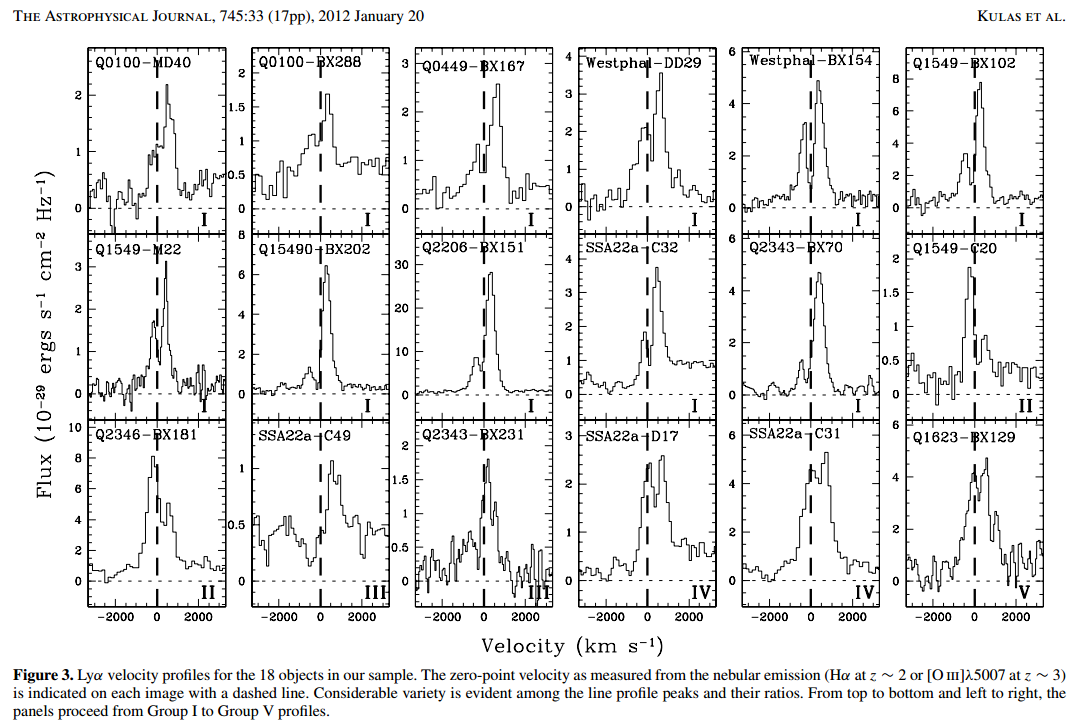
\includegraphics[width=1\textwidth]{./figures/chapter4/figure3}
	\end{center}
	\caption{\textbf{Figure 3 of Kulas et al. paper:} The Kinematics of Multiple-peaked \lya Emission in Star-forming Galaxies at $z\sim2-3$ \cite{Kulas12}. This plot is reproduced with the authors permission.
		\label{fig:kulas}}
\end{figure}
%http://arohatgi.info/WebPlotDigitizer/app/

The observed spectra in Fig. \ref{fig:kulas} are modified by the redshift $z$ of the galaxies. This is, how much distance light had to travel to reach their telescopes. That causes a broadening of the line. \\

Taking into account this effect, I notice similitudes between them and the simulated spectra. The \lya profiles are mostly 2 peaks with an asymmetry between them, just as in the simulation. Also, the small peak (if existing) is always smaller than the tall one.\\

Many authors that only include the outflows effect are able to fit observational spectra but with a very large magnitude of \vout, on the order of $50-100$ \kms. However, \vout is caused mainly by ejection of material out the galaxy. It is then common that a galaxy rotates faster than it expands, not the opposite. Other authors that include the rotational effect are able to obtain the two peaks but not their asymmetry. Simulating LAEs without outflows does not replicate the majority of the cases. \\

In my model, the combination of rotation and outflows velocities not only makes a lot of sense but seems to be able to fit observations. This new model proposed could replicate \lya profiles with typical LAE's values. The main result of this monograph is that I presented a new LAE model roughly consistent with observations.\\